\documentclass[11pt]{amsart}

\usepackage{tikz}
\usepackage{pgfplots}
\usepackage{amssymb}
\usepackage{amsmath}

\begin{document}

The power curve for any wind generation device will follow the general form:
\begin{equation}
P(v_{\mathrm{wind}}) = \min(k v_{\mathrm{wind}}^3, P_{\mathrm{rated}})
\end{equation}
In the $v_{\mathrm{wind}}^3$ section you're limited by the physics of
how much power is available in the wind.  Here, the coefficient $k$ is
determined by how large your wing or blade is and how efficiently it
is used.  On the other hand, in the flat section, the maximum power,
$P_{\mathrm{rated}}$, is determined by how large your generators and
inverters are.  For a given $P_{\mathrm{rated}}$, a larger $k$ will
result in a higher capacity factor, essentially because there is more
area under the power curve.  When you're comparing apples-to-apples
this is likely a good indication of how efficient your wind turbine
is.

\begin{center}
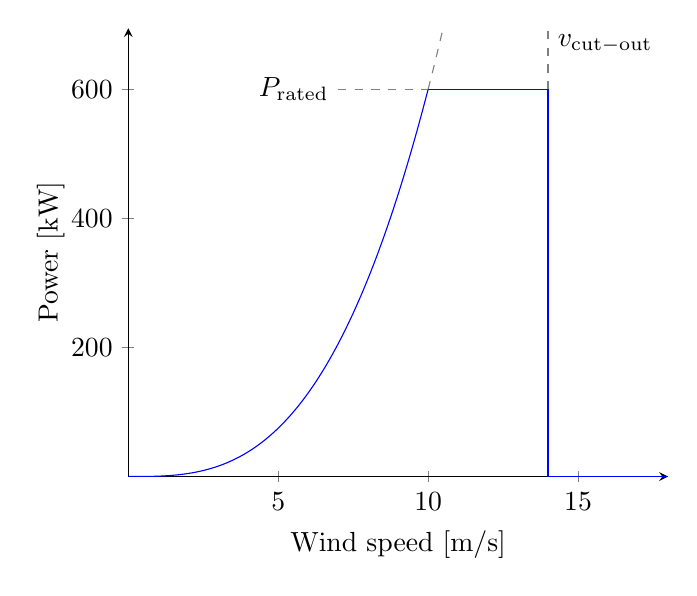
\begin{tikzpicture}
\begin{axis}[axis lines=middle, samples=200,
    x label style={at={(axis description cs:0.5,-0.1)}, anchor=north},
    y label style={at={(axis description cs:-0.1,.5)}, rotate=90, anchor=south},
    xlabel={Wind speed [m/s]},
    ylabel={Power [kW]}]
\addplot[blue, domain=0:10] {0.6 * x*x*x};
\addplot[gray, dashed, domain=10:10.5] {0.6 * x*x*x};

\draw[gray, dashed] (axis cs:7,600) node [left, black] {$P_{\mathrm{rated}}$} --
                    (axis cs:10,600);
\draw[blue] (axis cs:10,600) -- (axis cs:14,600);

\draw[gray, dashed] (axis cs:14,600) -- (axis cs:14,700) node [below right, black]
     {$v_{\mathrm{cut-out}}$};
\draw[blue] (axis cs:14,600) -- (axis cs:14,0);
\addplot[blue, domain=14:18] {0};
\end{axis}
\end{tikzpicture}
\end{center}

Since we aren't comparing apples-to-apples, we need to use a more
accurate metric, which takes cost into account.  In an extremely
simplified cost model, you could say that there is some cost per unit
$k$ and some cost per unit $P_{\mathrm{rated}}$.  (In reality, the
cost for $k$ probably grows as $k^{3/2}$ because $k$ grows as wing
area, whereas cost grows as wing mass.)
\begin{equation}
C(k, P_{\mathrm{rated}}) = c_k k + c_P P_{\mathrm{rated}}
\end{equation}
The optimization criterion for any wind generation device is to
maximize the ratio of the expected average power $\bar{P}$ over the
cost $C$.  In our system, $c_P$ is likely somewhat similar to
traditional wind turbines.  However, $c_k$ should be much less since
we are using the material so much more efficiently.  Because $k$ is
relatively cheaper for our system than $P_{\mathrm{rated}}$, we end up
with a little more of it.  This explains why, for a given
$P_{\mathrm{rated}}$, our system can have a larger $k$ and thus a high
capacity factor.

To make this concrete, let's play with a simple toy model where the
wind speed is distributed evenly between 0 and $v_{\mathrm{cut-out}}$.
Then the expected value of the power would be
\begin{eqnarray}
\bar{P} &=& \left[ \frac{1}{4} k v_{\mathrm{rated}}^4
  + P_{\mathrm{rated}} (v_{\mathrm{cut-out}} - v_{\mathrm{rated}}) \right]
  \Big/ v_{\mathrm{cut-out}} \\
       &=& P_{\mathrm{rated}} \left(1 - \frac{3}{4}
  \frac{(P_{\mathrm{rated}}/k)^{1/3}}{v_{\mathrm{cut-out}}} \right)
\end{eqnarray}
Then, our metric for performance is
\begin{equation}
\frac{\bar{P}}{C} = v_{\mathrm{rated}}^3 \cdot
\frac{1 - \frac{3}{4}\frac{v_{\mathrm{rated}}}{v_{\mathrm{cut-out}}}}{c_k + c_P \cdot v_{\mathrm{rated}}^3}
\end{equation}
which has a maximum when
\begin{equation}
\frac{c_P}{4 c_k} v_{\mathrm{rated}}^4 = v_{\mathrm{cut-out}} - v_{\mathrm{rated}}
\end{equation}
\begin{center}
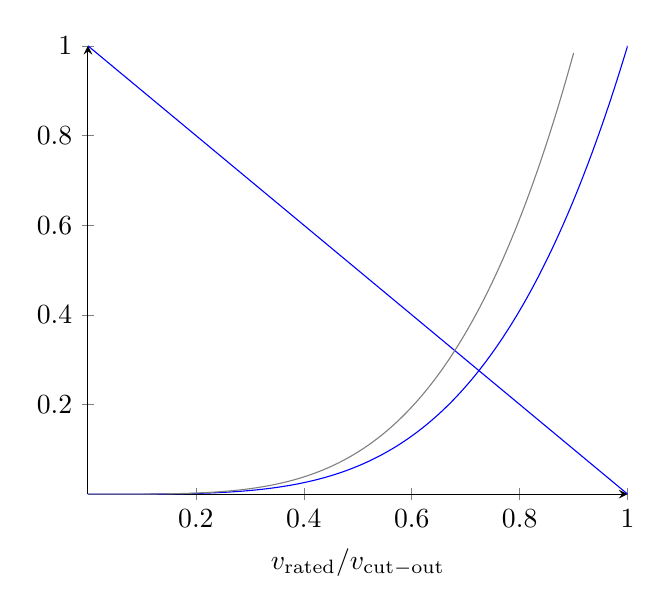
\begin{tikzpicture}
\begin{axis}[axis lines=middle, samples=200,
    x label style={at={(axis description cs:0.5,-0.1)}, anchor=north},
    y label style={at={(axis description cs:-0.1,.5)}, rotate=90, anchor=south},
    xlabel={$v_{\mathrm{rated}} / v_{\mathrm{cut-out}}$}]
\addplot[blue, domain=0:1] {1 - x};
\addplot[blue, domain=0:1] {x^4};
\addplot[gray, domain=0:0.9] {1.5 * x^4};
\end{axis}
\end{tikzpicture}
\end{center}
It's clear from the solution that a larger $\frac{c_P}{4c_k}$ results
in a lower $v_{\mathrm{rated}}$.  Or said another way, as structural
costs become cheaper it makes sense to reach the full rated power at
lower wind speeds.


\end{document}
